% Paper.tex
% Chrisna Aing, Sarah Halls, Kiva Oken
% OTTER COMPS!

\documentclass[12pt]{article}
\usepackage{amsmath}
\usepackage{amssymb}
\usepackage{graphicx}
\usepackage{multirow}
\usepackage[dvipsnames, table]{xcolor}
\usepackage[all]{xy}
\usepackage{hyperref}

\begin{document}

% This should be a lot prettier.
\title{Using Occupancy Theory and Hierarchical Models to Estimate Otter
Population in Southeastern Minnesota}
\date{}
\author{Chrisna Aing, Sarah Halls, Kiva Oken}
\maketitle

\section{Overview of occupancy modeling}

    \subsection{What is occupancy rate?}
    Occupancy has two different definitions. It can mean ``the probability that
    a randomly selected site or sampling unit in an area of interest is occupied
    by a species'' \cite{MacKenzie2006}. It also can be used to describe ``the
    proportion of area, patches, or sample units that is occupied''
    \cite{MacKenzie2006}. Occupancy is not the same as the abundance, or
    population size, of a species. The number of members of a species is not
    important for either definition of occupancy.

    While there is a difference between these two definitions of occupancy, in
    general the probability is unknown and the observed proportion is used as an
    estimate of the underlying probability. Because of this, these two
    definitions of occupancy are oftentimes used interchangeably.

    The main reasons that people are interested in measuring occupancy are
    science or conservation and management \cite{MacKenzie2006}. This statistic
    can give insight into the way a system works. It also can be used to monitor
    animals habitats and discover trends over time in groups of animals.

	
    \subsection{Different ways of sampling data}
    In order to determine occupancy rate, the data is often collected in the
    form of a presence-absence survey. This means that observers visit sites and
    look for the animals themselves, tracks, vocalizations, or some other
    indicator that the animal is present. In some cases, camera traps and sound
    recording are used instead of human observers \cite{MacKenzie2006}.

    The main problem with these methods of sampling data is that it is possible
    for an animal to occupy a site, but not be detected by the observer. This
    means that the site is recorded as unoccupied, but there really is an animal
    there. This is called a false negative. Marking an animal present when there
    really is no animal is also a possible problem, but is thought to be much
    less likely and is often ignored. We will discuss this issue more in later sections.

    \subsection{Assumptions}
    As is true for all modeling, there are some assumptions made in most models of occupancy 
in order to create simple enough models \cite{MacKenzie2006}. One common assumption is no false positives, which means if a
    site is recorded as occupied we say it must actually be occupied. A second
    common assumption is that presence and detection probabilities are constant
    across sites and surveys. This simplifies the estimation of each parameter.
    A third common assumption is that there is independence of detection between
    sites. A fourth common assumption is that the surveys are being conducted on
    a closed population. This means that no animals leave the area or joins the
    area during the time of the surveys.

    There are different methods for dealing with violations of these assumptions, some 
more developed than others.  In this paper, we will only talk about attempting to get rid of the
    assumption of no false positives and the assumption of independence of
    parameters across sites.

    \subsection{Types of occupancy models}
    All of the models discussed in this paper are single-species, single-season
    models. It is possible to modify all of these models to be used for multiple
    seasons or multiple species, at the cost of added complexity.

    The most simple way to measure occupancy is to simply divide the number of
    sites where an animal was found to be present by the total number of sites.
    This is called na\"ive occupancy \cite{MacKenzie2006}. It is generally
    accepted that this estimate is too low because animals are not detected at
    all sites where they are present, due to the issue of false negatives
    mentioned above. Other occupancy models attempt to do better than this
    simple estimate.

    One way to create a more accurate model is to attempt to model the biological 
proccess that is occuring.  In order to do this, we can use a Hierarchical model as a
    way to think about the parameters that affect occupancy. This allows us to
    take into account that when an animal is not detected, it could either not
    be there, or it could be there and just was not detected. This could either
    be due to a false negative, where the observer did not see the indication --
    for example they did not see the animal, track, etc. -- or it could be due
    to the fact that the animal does occupy the site but there was no indication
    of the animal at the site -- for example, no track, no vocalization, etc.

    Here is a visualization of how the Hierarchical model works:

    \begin{center}
        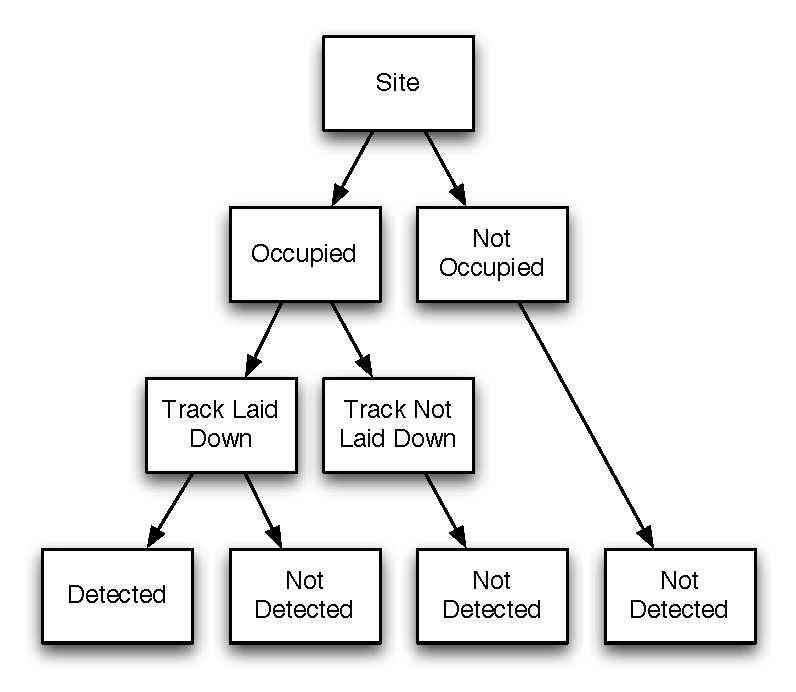
\includegraphics[scale=0.75]{SimpleHierarchicalModel}
    \end{center}

    From this diagram, it is apparent that we need separate parameters for the
    probability that a site is occupied, the probability that presence is
    indicated given that a site is occupied, and the probability of detection
    given that presence is indicated and the site is occupied. We will call
    these \(\psi\), \(\theta\), and \(p\), respectively.

\section{Questions of investigation}
The North American river otter (\textit{Lontra canadensis}) is endemic to all of
Minnesota; however, populations declined precipitously in the 19th and 20th
centuries due to trapping and habitat degradation. In recent years their
populations have significantly rebounded, especially in southeastern Minnesota
where hunters would like to be able to trap otters again. In order for that to
be possible governmental organizations must be able to monitor the population
health. In addition, otter presence can indicate high quality aquatic habitat.
Due to these reasons, there is interest in monitoring changes in otter abundance
over time. Unfortunately, otters are not easy to observe. Thus, this study
investigated the potential of using wintertime aerial surveys of otter tracks on
rivers to make inferences about the abundance of otters and how it changes over
time. We used the concepts from occupancy theory to develop models to estimate
the occupancy rate in order to get a sense of otter abundance.

    \subsection{Data collection}
    During the winters of 2003 and 2004 people flew over the Whitewater, Zumbro,
    and Mississippi Rivers. When they saw what looked like an otter track, they
    pushed a button recording the GPS coordinates. They pushed the button every
    five seconds until the track ended. Flights occurred one, two, or three days
    after a snow event. In some cases, multiple observers flew over the same
    river on the same day. Surveys were conducted during multiple snow events
    throughout both winters. The rivers were then divided into 400 and 800 meter
    plots and the presence (1) or absence (0) of a waypoint in a plot on a given
    flight was determined. The Mississippi River was also divided into 1600
    meter plots.

    \subsection{Issues related to the data}
    One major issue with respect to the data is that if a track occurred near
    the boundary between two plots, a person on one flight may have recorded the
    track in one site whereas someone on a later flight during that same snow
    event may have seen the same track but recorded it in the neighboring plot.
    So while the data indicate that the observers on the two flights disagreed
    in two plots, they saw the same track. Increasing the plot size should
    decrease the magnitude of this effect.

    In addition, there is concern that the probability of an otter laying down a
    track in one site is not independent of the probability that an otter lays
    down a track in neighboring sites, violating a principle assumption of
    occupancy theory. That is, a single track can extend across multiple plots.
    This leads to dependence among the plots. It was important to quantify this
    dependence and find an optimum way to handle it.

    \subsection{Descriptive statistics}
    In 2003, three different observers flew over the rivers. Assuming that no
    tracks are laid down between individuals' flights on the same day, all three
    people should have seen the same tracks. While there is some error in
    classifying in which plot the observer saw the actual track, each observer
    should at least be seeing the same, or nearly the same, number of sites with
    tracks. However, we did not find that to be the case. If we look only at
    days that all three people observed, there appear to be major differences
    among the proportion of sites in which the observers detected a track
    (Figure \ref{obsPlots}). The difference in estimated na\"ive occupancy among 
    the
    observers indicates that the observers did not always correctly identify
    the tracks.

    \begin{figure}
        	\centering
	    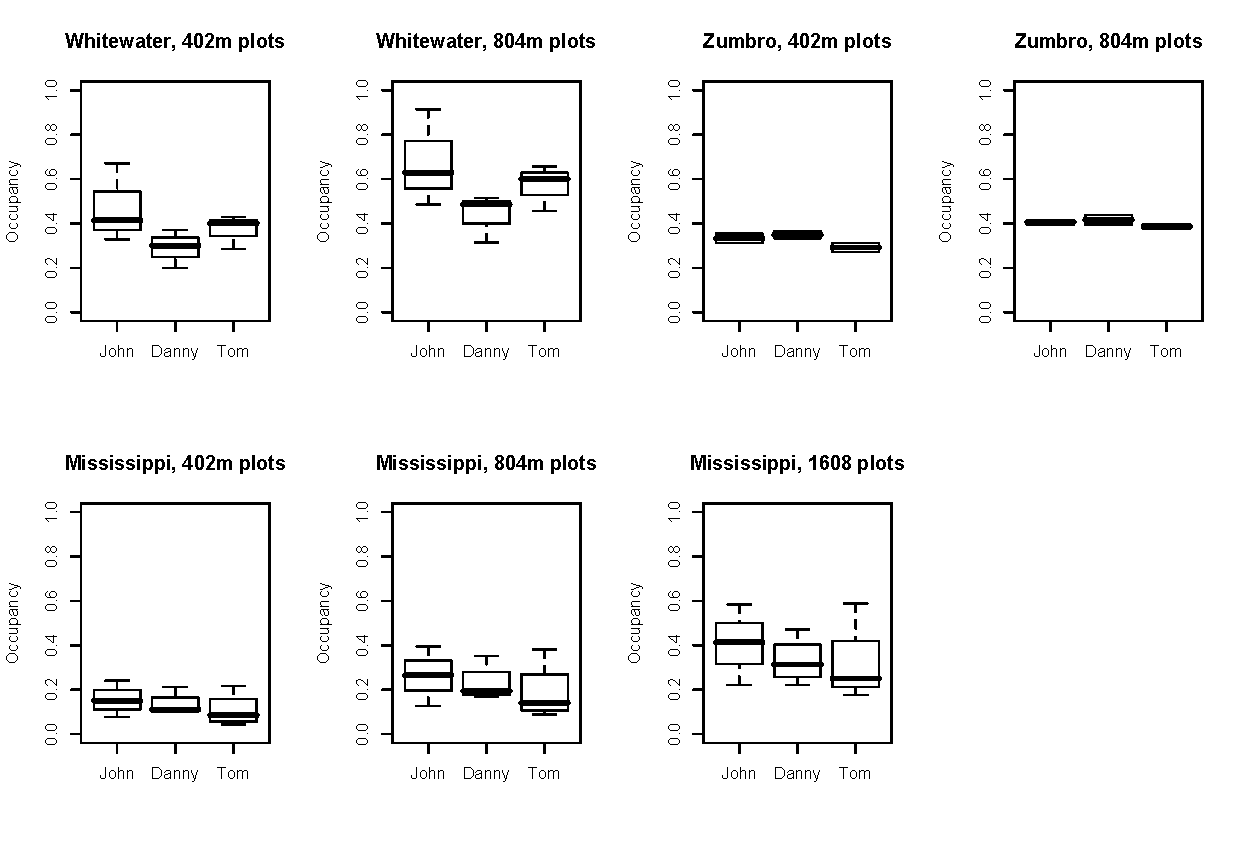
\includegraphics[width=5in]{observerPlots.pdf}
	    \caption{The box plots show how the proportion of sites in which an 
	    observer saw tracks (``occupancy'') differs among the three observers in 
	    2003. Only those dates on which all three observers flew are included.}
	    \label{obsPlots}
    \end{figure}

    Correlation among the flight sequences is low. For example, average
    correlation between flights on the Mississippi in 2003 is 0.176 for 400
    meter plots. Some of this is due to the difficulties in determining to which
    site each track belongs. However, we have also found quite a bit of
    variation in the data not necessarily due to these classification issues.
    This is difficult to quantify. Correlation between flights is a bit higher 
    for
    flights on the same day or flights during the same snow event, but still not
    as high as one might hope. Correlation rarely exceeds 0.5. The proportion of 
    sites with tracks detected
    generally increases with days since snow, likely because the otters have a
    longer time to lay down a track as time after the snow event passes.

    \subsection{False positive rates}
    The lack of consistency among the flights is strong evidence that the data
    contain false positives where observers think they see a track when it does
    not exist. Not accounting for such a process can lead to major biases; as
    the number of flights increases, the occupancy rate estimate will approach
    1 \cite{Royle2006}. Unlike most occupancy models where observers assume 
    that detection of the species in question guarantees its presence \cite
    {MacKenzie2006}, we introduced a false detection process whereby an observer 
    can mark down the existence of a track when in reality there is none. This 
    false detection process can occur as long as there is no track, whether or 
    not the site is occupied.

    \subsection{Testing the independence assumption}
    \label{shat}
    Since one of the assumptions of occupancy modeling is that there is 
	independence between sites, we wanted to see if this assumption held true 
	for our data.  In order to do this, we calculated the statistic \(S\), which
	we define as the number of successive \(0\), \(1\)'s minus the number of
    successive \(1\), \(1\)'s per flight. Under the null hypothesis that each
    site is an independent Bernoulli trial with probability of a \(1 = p\) we were able
    to compute the mean and standard deviation of \(S\), which we used to
    calculate a Z-score, where \(Z = (S – E[S])/SD[S]\). In order to compute these values, we needed to find the
    expected value and variance of each term in \(S\). These caclulations can be
	found in the appendix.  

    Simulations of \(S\) show that the distribution of \(S\) is roughly normal.
    So using our calculations for the mean and the standard deviation, we
    computed a Z-score for each flight, where we use a plug-in estimate for
    \(p\) to be the proportion of \(1\)'s per flight. We said that \(|Z| > 2\) suggests that the assumption of
    independence between sites is violated for that flight. We found that, in
    general, alternating sites are more "independent" than all sites as measured
    by this statistic. However, alternating sites do not guarantee independence.
    For instance, six of eleven flights along the Zumbro River during 2003 still
    have significant Z-scores with alternating sites. It also appears that there 
	may be slightly more independence when larger site sizes are used, although it is
not clear if this trend is significant.  There 
	were no noticable trends for this statistic with respect to observer, days 
	since snow, or snow event.

    % Mississippi River!
    \begin{center}
    \begin{tabular}{|l|l|l|l|l|l|}
        \hline
        \multicolumn{6}{|l|}{\textbf{Mississippi River}} \\
        \hline
        \multirow{2}{*}{Year} & \multirow{2}{*}{Size} & \multirow{2}{*}{Flights}
        & \multicolumn{2}{|l|}{\# Sig. Z-Scores} &
        \multirow{2}{*}{\(E[|z_{all}|-|z_{alt}|]\)} \\
        \cline{4-5}
        & & & All Plots & Alt. Plots & \\
        \hline
        \multirow{3}{*}{2003} & 402m & \multirow{3}{*}{20} & 7 & 0 & 0.915 \\
        \cline{2-2} \cline{4-6}
        & 804m & & 5 & 0 & 0.651 \\
        \cline{2-2} \cline{4-6}
        & 1608m & & 1 & 0 & 0.383 \\
        \hline
        \multirow{3}{*}{2004} & 402m & \multirow{3}{*}{6} & 5 & 3 & 0.625 \\
        \cline{2-2} \cline{4-6}
        & 804m & & 3 & 0 & 1.428 \\
        \cline{2-2} \cline{4-6}
        & 1608m & & 2 & 0 & 0.053 \\
        \hline
    \end{tabular}
    \end{center}

    % Whitewater River!
    \begin{center}
    \begin{tabular}{|l|l|l|l|l|l|}
        \hline
        \multicolumn{6}{|l|}{\textbf{Whitewater River}} \\
        \hline
        \multirow{2}{*}{Year} & \multirow{2}{*}{Size} & \multirow{2}{*}{Flights}
        & \multicolumn{2}{|l|}{\# Sig. Z-Scores} &
        \multirow{2}{*}{\(E[|z_{all}|-|z_{alt}|]\)} \\
        \cline{4-5}
        & & & All Plots & Alt. Plots & \\
        \hline
        \multirow{2}{*}{2003} & 402m & \multirow{2}{*}{15} & 6 & 2 & 0.722 \\
        \cline{2-2} \cline{4-6}
        & 804m & & 4 & 1 & 0.634 \\
        \hline
        \multirow{2}{*}{2004} & 402m & \multirow{2}{*}{6} & 3 & 1 & 1.189 \\
        \cline{2-2} \cline{4-6}
        & 804m & & 2 & 2 & 0.612 \\
        \hline
    \end{tabular}
    \end{center}

    % Zumbro River!
    \begin{center}
    \begin{tabular}{|l|l|l|l|l|l|}
        \hline
        \multicolumn{6}{|l|}{\textbf{Zumbro River}} \\
        \hline
        \multirow{2}{*}{Year} & \multirow{2}{*}{Size} & \multirow{2}{*}{Flights}
        & \multicolumn{2}{|l|}{\# Sig. Z-Scores} &
        \multirow{2}{*}{\(E[|z_{all}|-|z_{alt}|]\)} \\
        \cline{4-5}
        & & & All Plots & Alt. Plots & \\
        \hline
        \multirow{2}{*}{2003} & 402m & \multirow{2}{*}{11} & 10 & 6 & 1.883 \\
        \cline{2-2} \cline{4-6}
        & 804m & & 8 & 5 & 1.287 \\
        \hline
        \multirow{2}{*}{2004} & 402m & \multirow{2}{*}{4} & 3 & 3 & 2.425 \\
        \cline{2-2} \cline{4-6}
        & 804m & & 3 & 1 & 2.343 \\
        \hline
    \end{tabular}
    \end{center}

    We think that the lack of independence results from strings of ones where an
    otter left a track across multiple sites. When alternating sites are used,
    the strings are cut in half and the occurrence of \(1\), \(1\)'s is lower
    while the occurrence of \(0\), \(1\)'s stays about the same. It is
    noteworthy that virtually all the violations of independence are in the
    direction of more \(1\), \(1\)'s than would be expected. This reinforces our
    thoughts about successive \(1\)'s representing the same otter. We will
    discuss later whether this violation of independence actually matters in our
    model, and how this might affect the estimation of actual occupancy rates.

\section{Bayesian modeling theory and practice}

    \subsection{Bayesian statistics}
    Bayes' Theorem: \(P(\theta|X) = P(X|\theta)P(\theta) / P(X)\) \\

    This states that the posterior distribution \(\propto\) the likelihood
    \(\times\) the prior. Usually, the mean of the posterior distribution is
    then used as a point estimate for the parameter.

    We can use Bayesian statistics in the Hierarchical model as long as we set a
    prior for every parameter that we include. We can then use Markov Chain
    Monte Carlo (MCMC) to find a posterior distributions for every parameter. We
    run into a problem of duality with the probability of correct detection
    \(p\), and the probability of false detection \(E\). These two variables
    have bimodal posterior distributions, because \(p=x,E=y,\psi=z\) is the same
    as \(p=y,E=x,\psi=1-z\). Since we know that is reasonable for \(p\) to be
    greater than \(E\), we solved this problem by restricting the distribution
    of \(p\) to the range \(0.6\text{ to }1\), and \(E\) to \(0\text{ to }0.4\),  
    an approach recommended by Royle and Link \cite{Royle2006}. 

    \subsection{WinBUGS/R}
    To implement a Bayesian hierarchical model, we make use of the software
    packages WinBUGS \cite{Lunn2000}, R \cite{R2009}, BRugs \cite{Thomas2008},
    and, by extension, OpenBUGS \cite{Thomas2006}. One can describe the model
    using an ``intuitive `pseudo-code' representation'' in WinBUGS
    \cite{MacKenzie2006} and then run the model within the familiar environment
    of R using the combination of BRugs and OpenBUGS. OpenBUGS, the open source,
    cross-platform successor to WinBUGS, uses the same syntax. All of the
    aforementioned software packages are open source and available
    freely\footnote{WinBUGS: \url{http://www.mrc-bsu.cam.ac.uk/bugs/} and R:
    \url{http://www.r-project.org/} are available as standalone programs. The
    BRugs/OpenBUGS package can be installed by typing
    \texttt{install.packages("BRugs")} in R's interactive shell. Note that while
    R and OpenBUGS include official support for Mac OS X and Unix/Unix-like
    operating systems, WinBUGS and the BRugs package are only available for
    Windows.}.

    WinBUGS requires a representation of a model, data, and initial values on
    which a predetermined number of iterations of the MCMC algorithm are
    executed \cite{MacKenzie2006}.
    The data we received from the
    Minnesota Department of Natural Resources was not fixed with respect to
    our covariates and required us to implement one of the three common
    strategies used to deal with irregular datasets \cite{Spiegelhalter2003}.
    Our simulations, on the other
    hand, ran on datasets with a fixed number of observers, snow events, and
    observations after each snow event, which are much easier to implement
    within WinBUGS and R.

\section{Standard hierarchical model}

    \subsection{Our hierarchical model}
    For our model, we specified noninformative uniform \((0, 1)\) prior
    distributions for
    parameters \(\psi\) and \(\theta\), a common, natural choice given a lack of
    formal information about the prior or expert consensus \cite{MacKenzie2006}.
    We implemented models with normal and beta prior distributions on \(p\) and
    \(E\) and limited the range of \(p\) to the interval \((0.6, 1)\) and the
    range of \(E\) to the interval \((0, 0.4)\) in both models. We set the
    burn-in time for the MCMC simulation to 10,000 iterations. Each of these
    parameters are tracked and therefore are estimated. The covariates of this
    model are: observer, date, and the number of days since the last snow event.
    It was necessary to preprocess the Minnesota DNR's data to account for its
    irregularities.

    \subsection{Simulated data}
    We simulated both balanced and unbalanced datasets meant for the standard
    hierarchical model with given values of \(\psi\), \(\theta\), \(p\) for each
    observer, and \(E\) for each observer.  Balanced data sets, in this context,
    contain the same number of flights by the same observers after each snow
    event.  Naturally, unbalanced data sets do not.

    To simulate balanced data, we provided the following additional variables:
    the number of sites, the number of snow events, the number of observers, and
    the number of observations following each snow event. These variables are
    all that are required to allow us to generate data in which each snow event
    receives the same number of flights by the same number of observers, which
    greatly simplifies the accompanying hierarchical model. First, the
    simulation determines a site's occupancy based upon the given \(psi\) value.
    Then, for each day after each snow event, the simulation decides whether or
    not an otter laid down a track. For a given day after a snow event, a track
    is considered to be present if an otter lays a track down on any of the days
    after the snow event up to and including the given day.  Once that has been
    decided, the given \(p\) and \(E\) values are used to assign a 0 (not
    detected) or 1 (detected).

    Because of limitations with respect to WinBUGS' syntax, simulating
    unbalanced data requires much more additional information and a reformatting
    of the data as well as the corresponding hierarchical model. While the
    resulting code's structure differs significantly from that used for balanced
    data, the underlying model remains the same.

    To determine the efficacy of the standard model over the range of possible
    \(\psi\) and \(\theta\) values, we ran simulations with several combinations
    of \(\psi\) and \(\theta\), ran the model on each simulation, and compared
    the model's estimates to the simulation's parameters. The model with beta
    prior distributions on \(p\) and \(E\) performed better than the model with
    normal prior distributions on the same parameters. A table detailing the
    model's performance with the beta prior distributions lies below:

    \begin{center}
    \begin{tabular}{|l|l|l|l|}
        \hline
        \multicolumn{4}{|l|}{\textbf{The Model vs. Simulated Data}} \\
        \hline
            \(\psi\) & \(\theta\) & Convergence & 95\% CI (\(\psi\)) \\
        \hline
        \multirow{5}{*}{0.20}
            & \cellcolor{Green}0.20 & \cellcolor{Green}Good &
              \cellcolor{Green}(0.112, 0.305) \\
            & \cellcolor{Green}0.40 & \cellcolor{Green}Good &
              \cellcolor{Green}(0.142, 0.341) \\
            & \cellcolor{Green}0.60 & \cellcolor{Green}Good &
              \cellcolor{Green}(0.098, 0.284) \\
            & \cellcolor{Green}0.80 & \cellcolor{Green}Good &
              \cellcolor{Green}(0.097, 0.281) \\
            & \cellcolor{Yellow}1.00 & \cellcolor{Yellow}Okay &
              \cellcolor{Yellow}(0.117, 0.302) \\
        \hline
        \multirow{5}{*}{0.40}
            & \cellcolor{Yellow}0.20 & \cellcolor{Yellow}Okay &
              \cellcolor{Yellow}(0.388, 0.721) \\
            & \cellcolor{Green}0.40 & \cellcolor{Green}Good &
              \cellcolor{Green}(0.270, 0.494) \\
            & \cellcolor{Green}0.60 & \cellcolor{Green}Good &
              \cellcolor{Green}(0.287, 0.512) \\
            & \cellcolor{Red}0.80 & \cellcolor{Red}Bad &
              \cellcolor{Red}(0.277, 0.507) \\
            & \cellcolor{Yellow}1.00 & \cellcolor{Yellow}Okay &
              \cellcolor{Yellow}(0.279, 0.503) \\
        \hline
        \multirow{5}{*}{0.60}
            & \cellcolor{Yellow}0.20 & \cellcolor{Yellow}Good &
              \cellcolor{Yellow}(0.312, 0.581) \\
            & \cellcolor{Green}0.40 & \cellcolor{Green}Good &
              \cellcolor{Green}(0.400, 0.630) \\
            & \cellcolor{Yellow}0.60 & \cellcolor{Yellow}Okay &
              \cellcolor{Yellow}(0.462, 0.687) \\
            & \cellcolor{Yellow}0.80 & \cellcolor{Yellow}Okay &
              \cellcolor{Yellow}(0.502, 0.727) \\
            & \cellcolor{Red}1.00 & \cellcolor{Red}Bad &
              \cellcolor{Red}(0.318, 0.549) \\
        \hline
        \multirow{5}{*}{0.80}
            & \cellcolor{Green}0.20 & \cellcolor{Green}Good &
              \cellcolor{Green}(0.578, 0.838) \\
            & \cellcolor{Green}0.40 & \cellcolor{Green}Good &
              \cellcolor{Green}(0.736, 0.915) \\
            & \cellcolor{Yellow}0.60 & \cellcolor{Yellow}Okay &
              \cellcolor{Yellow}(0.587, 0.829) \\
            & \cellcolor{Yellow}0.80 & \cellcolor{Yellow}Okay &
              \cellcolor{Yellow}(0.599, 0.811) \\
            & \cellcolor{Red}1.00 & \cellcolor{Red}Bad &
              \cellcolor{Red}(0.612, 0.830) \\
        \hline
        \multirow{5}{*}{1.00}
            & \cellcolor{Yellow}0.20 & \cellcolor{Yellow}Good &
              \cellcolor{Yellow}(0.895, 0.999) \\
            & \cellcolor{Yellow}0.40 & \cellcolor{Yellow}Okay &
              \cellcolor{Yellow}(0.927, 0.999) \\
            & \cellcolor{Green}0.60 & \cellcolor{Green}Good &
              \cellcolor{Green}(0.949, 1.000) \\
            & \cellcolor{Yellow}0.80 & \cellcolor{Yellow}Good &
              \cellcolor{Yellow}(0.802, 0.954) \\
            & \cellcolor{Red}1.00 & \cellcolor{Red}Bad &
              \cellcolor{Red}(0.800, 0.955) \\
        \hline
    \end{tabular}
    \end{center}

    Each of the simulations represented in the table above ran with the
    following parameters: seventy sites, five snow events, three observers, and
    three observations after each snow event. The three observers had \(p\)
    values of 0.70, 0.80, 0.90 and \(E\) values of 0.05, 0.20, and 0.30,
    respectively.

    Green rows represent values of \(\psi\) and \(\theta\) for which our
    standard hierarchical model exhibits good convergence and provides a 95\%
    confidence interval for \(\psi\) that includes the simulated data's actual
    \(\psi\) value.  Yellow rows represent values of \(\psi\) and \(\theta\) for
    which our model exhibits either mediocre convergence with a good confidence
    interval or good convergence with a bad confidence interval.  Red rows
    represent values of \(\psi\) and \(\theta\) for which our model does not
    converge.  The 95\% confidence interval is ignored in these cases.

    Generally, the model is most effective for lower values of \(\psi\) and
    \(\theta\) but will either converge well or provide useful estimates for the
    vast majority of combinations of \(\psi\) and \(\theta\) values. 21 of the
    model's 25 confidence intervals for \(\psi\) include its actual value. With
    respect to \(p\), all of the model's confidence intervals for each of the
    three values of \(p\) include its actual value for all \(\psi\) and
    \(\theta\) values. On the other hand, the model accurately estimates \(E\)
    for low values of \(\theta\), but consistently overestimates \(E\) when
    \(\psi\geq0.4\) and \(\theta\geq0.6\) regardless of \(E\)'s actual value.

\section{Spatial correlation of the data}
One approach to dealing with the correlation in the probability of
observing a track in neighboring sites was to use a conditional autoregressive
(CAR) prior distribution for $\theta$, the probability that an otter lays down a
track in a site on a given day.

    \subsection{Conditional autoregressive (CAR) models}
    Let $\theta_s$ be the probability of a track being laid down in site $s$ on
    a given day. Then the Gaussian CAR model can be defined using the following
    conditional distributions:
    \begin{equation}
        \theta_s|\theta_i,\tau_s^2 \sim N(\mu_s+\sum_{i\in N_s}
        c_{si}(y_i-\mu_i),\tau_s^2)
    \end{equation}
    where $N_s$ is the set of neighbors of area $s$ (in this case, the two
    bordering sites), $E(\theta_s)=\mu_s$, $\tau_s^2$ is the conditional
    variance, $c_{si}$ is the weight defining how strong the correlation is
    between sites $s$ and $i$, and $c_{ii}=0$ for all sites $i$ \cite{Arab2008}.
    Essentially, this model means that if site $s$'s neighbor has a
    particularly high or low track-laying probability, that will increase or
    decrease the track-laying probability for site $s$. This makes it more
    likely to have strings of tracks that cross over multiple sites.

    \subsection{Our CAR model}
    \label{car model}
    For our model, both neighbors are weighted equally. Since $\tau_s$ for any
    site $s$ is unknown, we followed convention and used the same value of
    $\tau$ for all sites and placed a prior distribution on it. We chose a
    $\gamma(0.5,0.0005)$ prior distribution for $(\tau^2)^{-1}$, a common choice
    \cite{Thomas2004}. In our model we define $\text{logit}(\theta_s)=\alpha_0+
    \alpha_{1_s}$ where $\alpha_0$ has an improper uniform distribution and
    $\alpha_1$ has a Gaussian CAR distribution. We again used a uniform prior
    distribution on $\psi$ and the same beta prior distributions on $p$ and $E$.
    In this case, we limited the range of $p$ to the interval $(0.7,1)$ and the
    range of $E$ to $(0,0.3)$. We increased the burn-in time to 12,000
    iterations. With this model, instead of a single estimate for $\theta$ there
    are now $S$ estimates for $\theta$ where $S$ is the total number of sites.
    While ideally we would estimate an overall value for $\theta$, it seems more
    important for the purposes of this investigation to estimate $\psi$.

    \subsection{Simulating spatially correlated data}
    Because we modeled spatial correlation in $\theta$, we began by simulating
    spatial correlation in the track-laying process. To do this, we added an
    additional variable to the simulated data, $\alpha$. Under the new
    simulation method, $\theta$ is the probability of an otter laying down a
    track in site $i$ given site $i$ is occupied and site $i-1$ does
    \textit{not} have a track. If site $i$ is occupied and site $i-1$ does have
    a track, then the probability of an otter laying down a track in site $i$ is
    equal to $\theta+\alpha$. This means if there is a track in one site, there
    is more likely to be a track in the next site. However, when we ran data
    simulated using this new method on the model described in section \ref{car
    model}, the model almost never converged. We tested independence of the data
    using the $\hat{s}$ statistic we developed (section \ref{shat}) and found
    that the simulated data displayed much more independence than the actual
    data. We tried modeling spatial correlation in the occupancy process, $\psi
    $, instead of in the track-laying process, but the simulated data were again 
    more independent than the real data.

    To increase the correlation between sites we simulated data
    correlated in both the track-laying and occupancy processes. Under this 
    simulation method we
    again had the variables $\theta$ and $\alpha$, but we also had analogous
    variables $ \psi$ and $\beta$. In this case, $\psi$ is the probability an
    otter occupies site $i$ given that site $i-1$ is not occupied and $\psi+
    \beta$ is the probability that an otter occupies site $i$ given that site
    $i-1$ is occupied. With this increased spatial correlation we were able to
    more closely match the $\hat{s}$ $z$-scores found in the actual data. In
    addition, the CAR model converged more often with data simulated using this
    method, but it still did not converge consistently.

    When we ran the data with spatial correlation in the occupancy process on
    the CAR model, we could no longer compare the model estimate for $\psi$ to
    the simulated value of $\psi$ because they had different meanings. To get a
    sense of the overall occupancy rate in the simulated data we counted the
    number of sites that were occupied (known because the data are simulated)
    and divided that by the total number of sites. This proportion is the value
    we compared to the $\psi$ estimate from both hierarchical models.

\section{Discussion}

    \subsection{Obtaining convergence on the data}
    Recall that our standard hierarchical model contains the following
    parameters: \(\psi\) (the rate of occupancy), \(\theta\) (the probability of
    laying down a track given occupancy), \(p\) (the probability of detecting a
    track given that it is present, which is unique to each observer and makes
    \(1-p\) the false negative rate of detecting a track), and \(E\) (the false
    positive rate of detecting a track, which is unique to each observer).

    Once both the standard hierarchical model and the addition of a CAR prior
    distribution on \(\theta\) to the standard model exhibited convergence on
    our simulated data, we moved onto running both models on the data given to
    us by the Minnesota DNR. Recall that data was gathered during the winters of
    2003 and 2004 along the Mississippi, Whitewater, and Zumbro Rivers and
    aggregated with ArcGIS into vectors containing ones and zeroes representing
    the detection and non-detection of a track, respectively, within plots of
    length 402 meters, 804 meters, and 1608 meters. The covariates recorded
    were: the observer, the date, and the number of days since the last snow
    event. In general, the sparseness of the data gathered in 2004 caused us to
    simplify the model in order to obtain results. Unfortunately, the
    simplification results in estimates of \(\psi\) that do not seem accurate
    and are not directly comparable to estimates of \(\psi\) on 2003's data.

    The standard model converged reliably on all data gathered in 2003, but it
    did not converge on any of the data gathered in 2004. Considering that the
    amount of data gathered in 2004 pales in comparison to the amount of data
    gathered in 2003, this result was not surprising. The vast majority of
    2004's data consists of just one observer taking observations once after
    each snow event, which causes \(p\) and \(E\) in particular to not converge,
    regardless of plot size.

    To obtain convergence on 2004's relatively sparse data, we removed \(E\),
    which adds to the model the assumption that there are no false positives
    and, consequently, simplifies it greatly. Although the model still did not
    converge on data with plot sizes of 804m and 1608m, both the Whitewater and
    Zumbro Rivers' data at the 402m plot size converged. Although none of the
    Mississippi River's 2004 data converged, we still include estimates of
    \(p\), \(\psi\), and \(\theta\) at the 402m plot size to accompany the
    estimates corresponding to the Whitewater and Zumbro Rivers. For the most
    part, however, we feel that the absence of \(E\) from the model makes the
    the estimates of \(\psi\) much less dependable.

    The addition of a CAR prior distribution on \(\theta\) to the standard model
    caused the model to fail to converge on all of the data. Although the
    standard model and the CAR model performed similarly on simulated data
    whenever both models converged, the standard model converged much more often
    than did the CAR model. This is most likely due to the fact that the CAR
    model attempts to estimate too many parameters. Whereas the standard model
    estimates between eight and twelve parameters on the actual data (\(\psi\),
    \(\theta\), the four parameters of the beta distributions corresponding to
    \(p\) and \(E\), \(p\) for each observer, and \(E\) for each observer), the
    CAR model estimates \(\theta\) for each site. Because there are at least
    thirty-five sites in each data set (regardless of plot size), the CAR prior
    distribution adds a considerable amount of complexity to the model.

    We also tried to simplify this model by eliminating \(E\) because this was
    somewhat successful with respect to convergence with the standard model. We
    first attempted to fit this model to data from 2003 at the 402m plot size.
    Although the model successfully converged on all of this data, its estimates
    of \(\psi\), all of which were greater than 0.9, did not seem reasonable,
    especially in comparison to the standard model's estimates when given the
    same data. As a result, we did not attempt to fit this model to the rest of
    the data and do not include this model's estimates within our results.

    \subsection{Our estimates}
    Below, in tables, lie our estimates for all of the Minnesota DNR's data from
    2003 and 2004. Below each table is detailed commentary about the ability of
    the standard hierarchical model to converge, given the corresponding data.

    With respect to the model's ability to converge on the actual data, the most
    important factors are plot size, the number of flights recorded, and the
    number of estimated parameters. In general, both plot size and the number of
    flights recorded must be sufficiently small and large, respectively, for the
    standard model with \(E\) to converge.

    2003's data worked relatively well with the model. The presence of numerous
    observations that occur in the second and third days since the most recent
    snow event allows one of the more crucial assumptions of our hierarchical
    model -- that otter tracks laid on each day after a snow event are visible
    throughout the entire observation period and therefore, that it is more
    likely for an observer to detect a track on later days -- to be thoroughly
    tested. Most of the \(\psi\) and \(\theta\) estimates of 2003's data fall
    into ranges where our model is at its best, both with respect to convergence
    and to accurately estimating \(\psi\).

    2004's data, which suffered from the lack of multiple observers and
    observations later than one day after each snow event, does not provide
    enough data with respect to time (measured by the number of days since the
    last snow event) for the parameters \(p\) and \(E\) to converge, regardless
    of the number of Markov Chain Monte Carlo (MCMC) iterations performed.

    % Wow, this stuff SUCKS.
    As plot size increases, every estimated parameter tends to increase as well.
    Although the vast majority of these increases, even at the 1608m plot size,
    lie well within the 95\% confidence interval of the accompanying estimate at
    the 402m plot size, we believe that this trend makes sense. Only one track
    detection within a plot is necessary to assign it a 1. Therefore, once 402m
    plots are aggregated into 1608m plots, only one of the four 402m plots needs
    to be assigned a 1 in order for the entire 1608m plot to receive a 1. The
    amount of correlation between 1's determines the increase in the proportion
    of 1's to the number of plots -- as the amount of correlation increases, the
    increase in the proportion decreases.

    We believe that this increase leads to higher \(\psi\) and \(\theta\)
    estimates because the potential for multiple otters to lay tracks within the
    same plot increases. In southeastern Minnesota, most otters tolerate the
    presence of other otters in the areas they use most frequently, suggesting
    that they are neither solitary nor territorial \cite{Gorman2006}. This is
    consistent with the noticeable but modest increase in \(\theta\) across plot
    % I have no idea how to explain this... :(. sizes for all three rivers.
    However, estimates of \(\psi\) along the Whitewater and Zumbro Rivers remain
    constant, despite large increases in \(\theta\).

    % More detail, maybe?
    Similarly, the increases in estimates of \(p\) and \(E\) seem to result from
    the general increase of tracks laid per plot as the plot size grows. As plot
    size grows, the influence of a 1 increases, regardless of whether an otter
    track or a track from a different animal was observed.

    Lastly, we decided to use the data from every plot even though we believe
    that, as a result, our data violates the assumption of independence between
    sites. However, the model remains effective with spatially correlated data.
    Since the actual data is relatively sparse as it is, we consider the removal
    of half of it in order to preserve independence to be more harmful to the
    model than supplying it with correlated data. Therefore, all estimates come
    from all of the data that we were given.

    % Mississippi River!
    \begin{center}
    \begin{tabular}{|l|l|l|l|}
        \hline
        \multicolumn{4}{|l|}{\textbf{Mississippi River, 2003}} \\
        \hline
            & 402m & 804m & 1608m \\
        \hline
        \multirow{2}{*}{E[Danny]}
            & 0.01954 & 0.04808 & 0.06885 \\
            & (0.006515, 0.03663) & (0.01874, 0.08187) & (0.01778, 0.1383) \\
        \hline
        \multirow{2}{*}{E[John]}
            & 0.05216 & 0.07771 & 0.13650 \\
            & (0.027710, 0.07745) & (0.03881, 0.12100) & (0.03449, 0.2330) \\
        \hline
        \multirow{2}{*}{E[Tom]}
            & 0.02668 & 0.06140 & 0.10230 \\
            & (0.011990, 0.04622) & (0.02789, 0.10390) & (0.04287, 0.1796) \\
        \hline
        \multirow{2}{*}{p[Danny]}
            & 0.65240 & 0.67340 & 0.74960 \\
            & (0.548300, 0.75990) & (0.56760, 0.78290) & (0.60510, 0.8910) \\
        \hline
        \multirow{2}{*}{p[John]}
            & 0.67770 & 0.77580 & 0.82540 \\
            & (0.583500, 0.77280) & (0.66060, 0.88690) & (0.71390, 0.9326) \\
        \hline
        \multirow{2}{*}{p[Tom]}
            & 0.53670 & 0.54220 & 0.65330 \\
            & (0.501200, 0.61300) & (0.50160, 0.62850) & (0.51530, 0.8104) \\
        \hline
        \multirow{2}{*}{\(\psi\)}
            & 0.59380 & 0.69370 & 0.75820 \\
            & (0.439000, 0.75990) & (0.51800, 0.87380) & (0.54110, 0.9300) \\
        \hline
        \multirow{2}{*}{\(\theta\)}
            & 0.15280 & 0.20730 & 0.27690 \\
            & (0.111900, 0.19780) & (0.14580, 0.27390) & (0.19030, 0.3716) \\
        \hline
    \end{tabular}
    \end{center}

    This data converged well at the 402m and 804m plot sizes. At the 1608m plot
    size, \(E\), \(\psi\), and \(\theta\) did not converge well.

    \begin{center}
    \begin{tabular}{|l|l|}
        \hline
        \multicolumn{2}{|l|}{\textbf{Mississippi River, 2004}} \\
        \hline
            & 402m \\
        \hline
        \multirow{2}{*}{p[Danny]}
            & 0.3129 \\
            & (0.2174, 0.8107) \\
        \hline
        \multirow{2}{*}{\(\psi\)}
            & 0.7613 \\
            & (0.6609, 0.8833) \\
        \hline
        \multirow{2}{*}{\(\theta\)}
            & 0.8511 \\
            & (0.2426, 0.9973) \\
        \hline
    \end{tabular}
    \end{center}

    This data did not converge. We do not think that these estimates are
    accurate, but they are included for the sake of completeness.

    % Whitewater River!
    \begin{center}
    \begin{tabular}{|l|l|l|}
        \hline
        \multicolumn{3}{|l|}{\textbf{Whitewater River, 2003}} \\
        \hline
            & 402m & 804m \\
        \hline
        \multirow{2}{*}{E[Danny]}
            & 0.05608 & 0.0555 \\
            & (0.02474, 0.09554) & (0.002859, 0.1390) \\
        \hline
        \multirow{2}{*}{E[John]}
            & 0.16570 & 0.1931 \\
            & (0.10130, 0.23510) & (0.065910, 0.3384) \\
        \hline
        \multirow{2}{*}{E[Tom]}
            & 0.15350 & 0.2241 \\
            & (0.09758, 0.21660) & (0.110000, 0.3623) \\
        \hline
        \multirow{2}{*}{p[Danny]}
            & 0.66990 & 0.6985 \\
            & (0.56080, 0.79040) & (0.573100, 0.8366) \\
        \hline
        \multirow{2}{*}{p[John]}
            & 0.92040 & 0.9877 \\
            & (0.84270, 0.97590) & (0.945100, 1.0000) \\
        \hline
        \multirow{2}{*}{p[Tom]}
            & 0.75910 & 0.8575 \\
            & (0.65060, 0.85800) & (0.745400, 0.9600) \\
        \hline
        \multirow{2}{*}{\(\psi\)}
            & 0.87590 & 0.9126 \\
            & (0.72910, 0.98880) & (0.746900, 0.9955) \\
        \hline
        \multirow{2}{*}{\(\theta\)}
            & 0.24100 & 0.3779 \\
            & (0.17890, 0.30900) & (0.286500, 0.4721) \\
        \hline
    \end{tabular}
    \end{center}

    While the 402m data converged well, \(E\), \(\psi\), and \(\theta\) did not
    converge well for the 804m data.

    \begin{center}
    \begin{tabular}{|l|l|l|l|}
        \hline
        \multicolumn{2}{|l|}{\textbf{Whitewater River, 2004}} \\
        \hline
            & 402m \\
        \hline
        \multirow{2}{*}{p[Danny]}
            & 0.8237 \\
            & (0.5323, 0.9804) \\
        \hline
        \multirow{2}{*}{\(\psi\)}
            & 0.6066 \\
            & (0.4246, 0.8382) \\
        \hline
        \multirow{2}{*}{\(\theta\)}
            & 0.2068 \\
            & (0.1211, 0.3550) \\
        \hline
    \end{tabular}
    \end{center}

    This data converged well. However, we feel that the absence of \(E\) from
    the model makes the estimates much less dependable. The estimates are also
    much less precise than those from 2003 -- the confidence intervals of
    \(\psi\) and of \(p[Danny]\) are twice as large as those from 2003.

    % Zumbro River!
    \begin{center}
    \begin{tabular}{|l|l|l|}
        \hline
        \multicolumn{3}{|l|}{\textbf{Zumbro River, 2003}} \\
        \hline
            & 402m & 804m \\
        \hline
        \multirow{2}{*}{E[Danny]}
            & 0.02922 & 0.007066 \\
            & (0.006786, 0.05994) & (0.0000, 0.03403) \\
        \hline
        \multirow{2}{*}{E[John]}
            & 0.03388 & 0.008312 \\
            & (0.008584, 0.06880) & (0.0000, 0.04188) \\
        \hline
        \multirow{2}{*}{E[Tom]}
            & 0.02228 & 0.012960 \\
            & (0.002430, 0.05385) & (0.0000, 0.05642) \\
        \hline
        \multirow{2}{*}{p[Danny]}
            & 0.81890 & 0.837100 \\
            & (0.749500, 0.88540) & (0.7615, 0.90700) \\
        \hline
        \multirow{2}{*}{p[John]}
            & 0.81770 & 0.852500 \\
            & (0.740100, 0.88670) & (0.7597, 0.92230) \\
        \hline
        \multirow{2}{*}{p[Tom]}
            & 0.73120 & 0.805400 \\
            & (0.625400, 0.82440) & (0.6885, 0.89780) \\
        \hline
        \multirow{2}{*}{\(\psi\)}
            & 0.66550 & 0.651600 \\
            & (0.549100, 0.78150) & (0.5098, 0.78210) \\
        \hline
        \multirow{2}{*}{\(\theta\)}
            & 0.29950 & 0.395800 \\
            & (0.236400, 0.36550) & (0.3100, 0.48520) \\
        \hline
    \end{tabular}
    \end{center}

    Again, the 402m data converged well. With respect to the 804m data, while
    \(\psi\) and \(\theta\) converged well, none of the other parameters did.

    \begin{center}
    \begin{tabular}{|l|l|l|l|}
        \hline
        \multicolumn{2}{|l|}{\textbf{Zumbro River, 2004}} \\
        \hline
            & 402m \\
        \hline
        \multirow{2}{*}{p[Danny]}
            & 0.9166 \\
            & (0.7739, 0.9918) \\
        \hline
        \multirow{2}{*}{\(\psi\)}
            & 0.4773 \\
            & (0.3586, 0.6114) \\
        \hline
        \multirow{2}{*}{\(\theta\)}
            & 0.4232 \\
            & (0.3073, 0.5520) \\
        \hline
    \end{tabular}
    \end{center}

    This data converged well. However, as is the case with all of the 2004 data,
    we feel that the absence of \(E\) from the model makes the estimates much
    less dependable.

    \subsection{Covariates}
    To determine the relative importance of our covariates (observer, date, and
    number of days since the most recent snow event), we ran the standard
    hierarchical model with \(E\) on simulated data with values of \(\psi\) and
    \(\theta\) similar to our estimates of \(\psi\) and \(\theta\) on 2003's
    data with varying numbers of observers, snow events, and observations after
    each snow event. We assume that observations after each snow event will
    occur on consecutive days, starting from the first day after the snow event.
    This information helped us to find the most efficient ways (with respect to
    number of flights) to gather aerial occupancy data given one, two, and three
    observers while still obtaining useful estimates from the model.

    The number of observers proved to be the least important of the three
    covariates. We were able to obtain accurate estimates regardless of the
    number of observers, as long as there were sufficient numbers of snow events
    and observations after each snow event. For one observer, at least three
    snow events and three observations on consecutive days after each snow event
    are required for the model to converge and give good estimates. For two or
    three observers, two events with three observations on consecutive days
    after each snow event is sufficient. Therefore, roughly nine, twelve, and
    eighteen flights are required to obtain good estimates for one, two, and
    three observers, respectively. Surprisingly, the most cost-effective method
    (as measured by the number of flights required) only requires one observer.

    The number of snow events proved to be the second-most important of the
    three covariates. Although two snow events are required, only with one
    observer does the addition of a third snow event noticeably affect the
    model's estimates.

    The number of observations after each snow event proved to be the most
    important of the three covariates. Because the model relies upon the
    assumption that the probability of seeing a track increases each day because
    tracks made on previous days within the same snow event can still be seen,
    this is not surprising. Two observations after each snow event on
    consecutive days are required. Additional observations after each event help
    the model converge more quickly, but the estimates become only slightly more
    accurate.

    \subsection{Future work}
    Additional observations are more helpful than additional snow events at
    first, although both are much more helpful than the addition of an observer.
    Once the numbers of snow events and observations after each snow event both
    surpass three, they improve the model's estimates at roughly equal rates.
    Note, however, that increasing the number of snow events is likely to be far
    less challenging than increasing the number of observations after each snow
    event at that point, especially in southeastern Minnesota.

    In summary, for future data gathering trips, we strongly suggest using one
    observer, as long as they are relatively confident that they can correctly
    identify an otter track and distinguish an otter track from the tracks of
    other animals in the immediate area, since the model most accurately
    estimates \(p\) and \(E\) when their true values are high and low,
    respectively. With one observer, three snow events and three or four snow
    days' worth of flights per snow event would be sufficient. If the same
    observer flies twice (or more often) in one day, perhaps they could act as a
    substitute for an additional observer. This is because it is probable that,
    with one flight's worth of experience observing the given river, the
    observer's \(p\) and \(E\) would change due to their newfound familiarity
    with the river.

\section{Acknowledgments}
We would like to thank our adviser, Bob Dobrow, for all of his help and advice and John Fieberg and John Erb from the Minnesota Department of Natural Resources for collecting and sharing the data as well as for offering their specific knowledge of the subject.

\bibliographystyle{amsplain}
\bibliography{Bibliography}

%Needs to be fixed/formatted better... I didn't know how to make an appendix
\appendix
	We let \(A = \text{\# of
    0-1's}\), \(B=\text{\# of 1-1's}\) and \(p=P(``1")\text{ in the sequence}\).
    In order to find \(E[s]\), we first needed to find \(E[A]\) and
    \(E[B]\).

    % E[A]
    \begin{equation*}
        \begin{split}
        E[A]& =\sum_{i=1}^{n-1}P(X_i=0,X_{i+1}=1) \\
            & =\sum_{i=1}^{n-1}(1-p)p \\
            & =(n-1)(1-p)p \\
        \end{split}
    \end{equation*}

    % E[B]
    \begin{equation*}
        \begin{split}
        E[B]& =\sum_{i=1}^{n-1}P(X_i=1,X_{i+1}=1) \\
            & =\sum_{i=1}^{n-1}p*p \\
            & =(n-1)p^2
        \end{split}
    \end{equation*}

    % E[s]
    \begin{equation*}
        \begin{split}
        E[s]& =E[A]-E[B] \\
                  & =(n-1)\left((1-p)p-p^2\right)
        \end{split}
    \end{equation*}

    The standard deviation was a little more difficult.  

    % Var[A]
    \begin{equation*}
        \begin{split}
        Var[A]& =\sum_{i=1}^{n-1}Var[A]+2\sum_{i=1}^{n-2}Cov[I_i=(0,1),I_{i+1}=
                 (1,1)] \\
              & =(n-1)P((0,1))(1-P((0,1))) \\
              & \quad +2\sum_{i=1}^{n-2}\bigg(E[I_i=(0,1),I_{i+1}=(0,1)]-E[I_i=
                (0,1)]E[I_{i+1}=(0,1)]\bigg) \\
              & =(n-1)(1-p)p(1-(1-p)p)+2\sum_{i=1}^{n-2}\bigg(0-(1-p)p(1-p)p
                \bigg) \\
              & =(1-p)p(-1+n+5p-3np-5p^2+3np^2)
        \end{split}
    \end{equation*}

    % Var[B]
    \begin{equation*}
        \begin{split}
        Var[B]& =\sum_{i=1}^{n-1}Var[B]+2\sum_{i=1}^{n-2}Cov[I_i=(1,1),I_{i+1}=
                (1,1)] \\
              & =(n-1)P((1, 1))(1-P((1, 1))) \\
              & \quad +2\sum_{i=1}^{n-2}\bigg(E[I_i=(1,1),I_{i+1}=(1,1)]-E[I_i=
                (1,1)]E[I_{i+1}=(1,1)]\bigg) \\
              & =(n-1)p^2(1-p^2)+2(n-2)(p^3-p^4) \\
              & =(1-p)p^2(-1+n-5p+3np)
        \end{split}
    \end{equation*}

    % Cov[A, B]
    \begin{equation*}
        \begin{split}
        Cov[A,B]& =\sum_{i=1}^{n-1}\sum_{j=1}^{n-1}Cov[A,B] \\
                & =\sum_{i=1}^{n-2}Cov[A,B]+\sum_{i=1}^{n-2}Cov[B,A] \\
                & \quad +\sum_{i=1}^{n-1}Cov[X_i=0\text{ or }1,X_{i+1}=1] \\
                & =\sum_{i=1}^{n-2}E[AB]-E[A]E[B]+\sum_{i=1}^{n-2}E[BA]-
                  E[B]E[A] \\
                & \quad +\sum_{i=1}^{n-1}E[X_i=0\text{ or }1,X_{i+1}=1]-
                  E[B]E[A] \\
                & =(n-2)(p-1)^2p^2-(n-2)p^3(1-p)-(n-1)p^3(1-p)
        \end{split}
    \end{equation*}

    % Var[s]
    \begin{equation*}
        \begin{split}
        Var[s]& =Var[A-B] \\
                    & =Var[A]+Var[B]-2Cov[A,B] \\
                    & =(1-p)p(-1+n+8p-4np-20p^2+12np^2)
        \end{split}
    \end{equation*}

\end{document}